\documentclass{beamer}
\usepackage{beamerthemesplit}
\usepackage{wrapfig}
\usetheme{SPbGU}
\usepackage{pdfpages}
\usepackage{amsmath}
\usepackage{cmap} 
\usepackage[T2A]{fontenc} 
\usepackage[utf8]{inputenc}
\usepackage[english,russian]{babel}
\usepackage{indentfirst}
\usepackage{amsmath}
\usepackage{tikz}
\usepackage{dot2texi}
\usepackage{multirow}
\usepackage{fancyvrb}
\usepackage{graphicx}
\usepackage{array}
\usepackage{subcaption}
\usepackage[noend]{algpseudocode}
\usepackage{algorithm}
\usepackage{algorithmicx}
\usetikzlibrary{shapes,arrows}
\usepackage{fancyvrb}
\usepackage[normalem]{ulem} % для подчёркиваний uline
\newtheorem{rutheorem}{Теорема}
\newtheorem{ruproof}{Доказательство}
\newtheorem{rudefinition}{Определение}
\newtheorem{rulemma}{Лемма}
\beamertemplatenavigationsymbolsempty


\title[]{Синтаксический анализ графов через умножение матриц}
\subtitle[]{В рамках проекта лаборатории JetBrains}
% То, что в квадратных скобках, отображается в левом нижнем углу. 
\institute[СПбГУ]{
	Санкт-Петербургский Государственный Университет \\
	Кафедра системного программирования }

% То, что в квадратных скобках, отображается в левом нижнем углу.
\author[Рустам Азимов]{Рустам Шухратуллович Азимов, 646 группа \\
	% У научного руководителя должна быть указана научная степень
	\and  
	{\bfseries Научный руководитель:} к.ф.-м.н., доцент С.В. Григорьев \\ 
	% Для курсовой не обязателен. Должна быть указана должность или ученая степень
	\and
	{\bfseries Рецензент:} преподаватель, научный координатор Академии Або и Центра Компьютерных Наук TUCS М.Л. Бараш}

\date{28 марта 2018г.}

\definecolor{orange}{RGB}{179,36,31}

\begin{document}
{
% Лого университета или организации, отображается в шапке титульного листа
\begin{frame}
  \titlepage
\end{frame}
}

\begin{frame}[fragile]
	\transwipe[direction=90]
	\frametitle{Синтаксический анализ графов}
	\begin{itemize}
	   \item Вход:
	   \begin{itemize}
	        \item Ориентированный граф D = (V,E) с метками на ребрах из алфавита $\Sigma$
	        \item КС-грамматика (запрос к графу) $G = (\Sigma,N,P)$ над тем же алфавитом
	   \end{itemize}
	   \item Выход для реляционной семантики запросов:
	   \begin{itemize}
	        \item Множество всех троек $(A, m, n)$, где существует путь из вершины $m$ в вершину $n$, метки на ребрах которого образуют строку, выводимую из нетерминала $A$
	   \end{itemize}
   	   \item Выход для single-path семантики запросов:
   	   \begin{itemize}
   			\item Дополнительно предоставить один такой путь для каждой тройки $(A, m, n)$
   	   \end{itemize}
    \end{itemize}
\end{frame}

\begin{frame}[fragile]
	\transwipe[direction=90]
	\frametitle{Пример}
\begin{figure}[h]
   \[
\begin{array}{rccl}
   0: & S & \rightarrow & \text{\textit{subClassOf}}^{-1} \ S \ \text{\textit{subClassOf}} \\ 
   1: & S & \rightarrow & \text{\textit{type}}^{-1} \ S \ \text{\textit{type}} \\ 
   2: & S & \rightarrow & \text{\textit{subClassOf}}^{-1} \ \text{\textit{subClassOf}} \\ 
   3: & S & \rightarrow & \text{\textit{type}}^{-1} \ \text{\textit{type}} \\ 
\end{array}
\]
\caption{Пример входной грамматики}
\label{ProductionRulesExampleQuery}
\end{figure}

\begin{figure}[h]
\[
    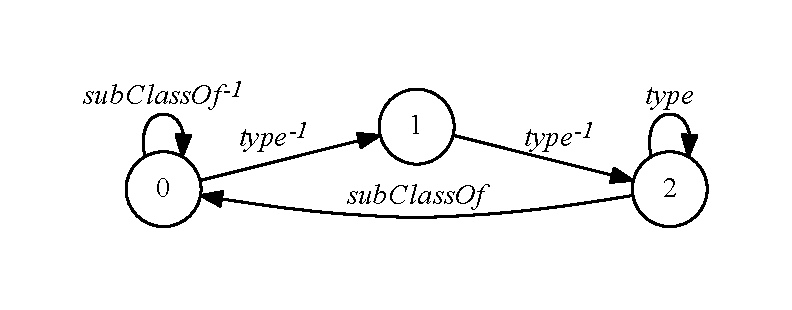
\includegraphics[width=8cm]{pictures/ExampleGraph.pdf}
\]
\caption{Пример входного графа}
\label{ExampleQueryGraph}
\end{figure}
\end{frame}
            
\begin{frame}[fragile]
	\transwipe[direction=90]
	\frametitle{Применимость}
	\begin{itemize}
	   \item Запросы к графовым базам данных
	   \item Анализ RDF файлов
	   \item Биоинформатика
	   \item Статический анализ программ
    \end{itemize}
\end{frame}

\begin{frame}[fragile]
	\transwipe[direction=90]
	\frametitle{Существующие алгоритмы}
	\begin{itemize}
	   \item Реляционная семантика запросов
	   \begin{itemize}
	   	\item Основанный на CYK (J. Hellings, 2014) 
	   	\item Тот же алгоритм, реализованный для анализа RDF файлов (X. Zhang, Z. Feng, X. Wang et al., 2016)
	   \end{itemize}
   		\item Single-path семантика запросов
   	   \begin{itemize}
   	   	\item Основанный на методе динамического программирования (J. Hellings, 2015) 
   	   	\item Основанный на GLL (Григорьев Семен, Рогозина Анастасия, 2016)
   	   \end{itemize} 
	   
    \end{itemize}
\end{frame}

\begin{frame}[fragile]
	\transwipe[direction=90]
	\frametitle{Проблемы}
	\begin{itemize}
		\item Низкая производительность на больших графах
		\item Существующие алгоритмы не позволяют эффективно применить такие техники, как вычисление на графическом процессоре, параллельное вычисление
	   \item Возможность создания матричного алгоритма синтаксического анализа графов является открытой проблемой
    \end{itemize}
\end{frame}

\begin{frame}[fragile]
\transwipe[direction=90]
\frametitle{Постановка задачи}
\textbf{Цель}: Разработать эффективный матричный алгоритм синтаксического анализа графов

\textbf{Задачи}:
\begin{itemize}
	\item Разработать матричный алгоритм синтаксического анализа графов для реляционной семантики запросов
	\item Разработать матричный алгоритм синтаксического анализа графов для single-path семантики запросов
	\item Показать практическую применимость предложенных алгоритмов на общепринятом наборе данных
\end{itemize}
\end{frame}

\begin{frame}[fragile]
	\transwipe[direction=90]
	\frametitle{Результаты}
	\begin{itemize}
	   \item Предложены алгоритмы синтаксического анализа графов, вычисляющие матричное транзитивное замыкание
	   \item Доказана корректность предложенных алгоритмов
	   \item Алгоритмы реализованы с использованием комбинаций таких оптимизаций, как:
	   \begin{itemize}
	    \item Разреженное представление матриц
	    \item Умножение матриц на графическом процессоре
	    \item Параллельное умножение матриц
	   \end{itemize}
	   \item Проведена апробация на общепринятом наборе RDF файлов
    \end{itemize}
\end{frame}

\begin{frame}[fragile]
	\transwipe[direction=90]
	\frametitle{Пример работы алгоритма}
\begin{figure}[h]
   \[
\begin{array}{rccl}
   0: & S & \rightarrow & \text{\textit{subClassOf}}^{-1} \ S \ \text{\textit{subClassOf}} \\ 
   1: & S & \rightarrow & \text{\textit{type}}^{-1} \ S \ \text{\textit{type}} \\ 
   2: & S & \rightarrow & \text{\textit{subClassOf}}^{-1} \ \text{\textit{subClassOf}} \\ 
   3: & S & \rightarrow & \text{\textit{type}}^{-1} \ \text{\textit{type}} \\ 
\end{array}
\]
\caption{Пример входной грамматики}
\label{ProductionRulesExampleQuery}
\end{figure}

\begin{figure}[h]
\[
    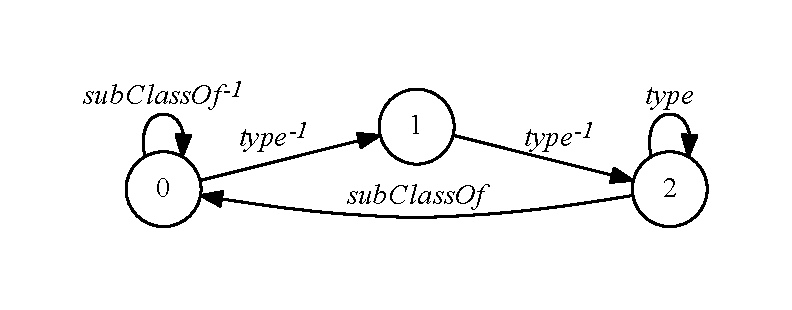
\includegraphics[width=8cm]{pictures/ExampleGraph.pdf}
\]
\caption{Пример входного графа}
\label{ExampleQueryGraph}
\end{figure}
\end{frame}

\begin{frame}[fragile]
	\transwipe[direction=90]
	\frametitle{Пример: Грамматика в нормальной форме}
\begin{figure}[h]
   \[
\begin{array}{rccl}
   0: & S & \rightarrow & S_1 \ S_5 \\
   1: & S & \rightarrow & S_3 \ S_6 \\
   2: & S & \rightarrow & S_1 \ S_2 \\
   3: & S & \rightarrow & S_3 \ S_4 \\
   4: & S_5 & \rightarrow & S \ S_2 \\
   5: & S_6 & \rightarrow & S \ S_4 \\
   6: & S_1 & \rightarrow & \text{\textit{subClassOf}}^{-1} \\ 
   7: & S_2 & \rightarrow & \text{\textit{subClassOf}} \\ 
   8: & S_3 & \rightarrow & \text{\textit{type}}^{-1} \\
   9: & S_4 & \rightarrow & \text{\textit{type}} \\ 
\end{array}
\]
\caption{Входная грамматика в нормальной форме Хомского}
\label{ProductionRulesExampleQueryCNF}
\end{figure}
\end{frame}

\begin{frame}[fragile]
	\transwipe[direction=90]
	\frametitle{Пример: Начальная матрица и первая итерация}
\begin{figure}[h]
\[
T_0 = \begin{pmatrix}
    \{S_1\} & \{S_3\} & \varnothing \\ \varnothing & \varnothing & \{S_3\} \\ \{S_2\} & \varnothing & \{S_4\}
\end{pmatrix}
\]
\caption{Начальная матрица}
\label{ExampleQueryInitMatrix}
\end{figure}

\begin{figure}[h]
\[
T_0 \cdot T_0 = \begin{pmatrix}
    \varnothing & \varnothing & \varnothing \\ \varnothing & \varnothing & \{S\} \\ \varnothing & \varnothing & \varnothing
\end{pmatrix}
\]

\[
T_1 = T_0 \cup (T_0 \cdot T_0) = \begin{pmatrix}
    \{S_1\} & \{S_3\} & \varnothing \\ \varnothing & \varnothing & \{S_3, S\} \\ \{S_2\} & \varnothing & \{S_4\}
\end{pmatrix}
\]
\caption{Первая итерация вычисления матричного транзитивного замыкания}
\label{ExampleQueryFirstIteration}
\end{figure}
\end{frame}

\begin{frame}[fragile]
	\transwipe[direction=90]
	\frametitle{Пример: Остальные итерации}
\begin{figure}[h]
\[
T_2 = \begin{pmatrix}
    \{S_1\} & \{S_3\} & \varnothing \\ \{S_5\} & \varnothing & \{S_3, S, S_6\} \\ \{S_2\} & \varnothing & \{S_4\}
\end{pmatrix}
\]

\[
T_3 = \begin{pmatrix}
    \{S_1\} & \{S_3\} & \{S\} \\ \{S_5\} & \varnothing & \{S_3, S, S_6\} \\ \{S_2\} & \varnothing & \{S_4\}
\end{pmatrix}
\]

\[
T_4 = \begin{pmatrix}
    \{S_1, S_5\} & \{S_3\} & \{S, S_6\} \\ \{S_5\} & \varnothing & \{S_3, S, S_6\} \\ \{S_2\} & \varnothing & \{S_4\}
\end{pmatrix}
\]

\[
T_5 = \begin{pmatrix}
    \{S_1, S_5, S\} & \{S_3\} & \{S, S_6\} \\ \{S_5\} & \varnothing & \{S_3, S, S_6\} \\ \{S_2\} & \varnothing & \{S_4\}
\end{pmatrix}
\]
\caption{Остальные состояния матрицы $T$.}
\label{ExampleQueryFinalIterations}
\end{figure}
\end{frame}

\begin{frame}[fragile]
	\transwipe[direction=90]
	\frametitle{Пример: Результирующие отношения по матрице $T_6 = T_5$}
\begin{figure}[h]
\begin{eqnarray*}
R_S&=&\{(0,0),(0,2),(1,2)\},\\
R_{S_1}&=&\{(0,0)\},\\
R_{S_2}&=&\{(2,0)\}, \\
R_{S_3}&=&\{(0,1), (1,2)\}, \\
R_{S_4}&=&\{(2,2)\}, \\
R_{S_5}&=&\{(0,0), (1,0)\}, \\
R_{S_6}&=&\{(0,2), (1,2)\}.
\end{eqnarray*}
\caption{Результирующие КС-отношения}
\label{ExampleQueryCFRelations}
\end{figure}
\end{frame}

\begin{frame}[fragile]
	\transwipe[direction=90]
	\frametitle{Апробация: Запрос 1}
\begin{figure}[h]
   \[
\begin{array}{rccl}
   0: & S & \rightarrow & \text{\textit{subClassOf}}^{-1} \ S \ \text{\textit{subClassOf}} \\ 
   1: & S & \rightarrow & \text{\textit{type}}^{-1} \ S \ \text{\textit{type}} \\ 
   2: & S & \rightarrow & \text{\textit{subClassOf}}^{-1} \ \text{\textit{subClassOf}} \\ 
   3: & S & \rightarrow & \text{\textit{type}}^{-1} \ \text{\textit{type}} \\ 
\end{array}
\]
\caption{Грамматика для запроса 1}
\label{ProductionRulesQuery1}
\end{figure}
\end{frame}

\begin{frame}[fragile]
  \transwipe[direction=90]
  \frametitle{Апробация: результаты для запроса 1}
\begin{center}
\begin{tabular}{ | c | c | c | c | c | c | c |}
\hline
Ontology & edgs & result & GLL & dGPU & sCPU & sGPU \\
\hline 
\hline
skos        & 252 & 810 & 10 & 56 & 14 & 12\\
generations & 273 & 2164 & 19 & 62 & 20 & 13\\
travel      & 277 & 2499 & 24 & 69 & 22 & 30\\
univ-bench  & 293 & 2540 & 25 & 81 & 25 & 15\\
atom-primitive & 425 & 15454 & 255 & 190 & 92 & 22\\
biomedical & 459 & 15156 & 261 & 266 & 113 & 20\\
foaf        & 631 & 4118 & 39 & 154 & 48 & 9\\
people-pets & 640 & 9472 & 89 & 392 & 142 & 32\\
funding     & 1086 & 17634 & 212 & 1410 & 447 & 36\\
wine        & 1839 & 66572 & 819 & 2047 & 797 & 54\\
pizza       & 1980 & 56195 & 697 & 1104 & 430 & 24\\
$g_{1}$     & 8688 & 141072 & 1926 & --- & 26957 & 82\\
$g_{2}$     & 14712 & 532576 & 6246 & --- & 46809 & 185\\
$g_{3}$     & 15840 & 449560 & 7014 & --- & 24967 & 127\\
\hline
\end{tabular}
\end{center}  
\end{frame}

\begin{frame}[fragile]
	\transwipe[direction=90]
	\frametitle{Апробация: Запрос 2}
\begin{figure}[h]
   \[
\begin{array}{rccl}
   0: & S & \rightarrow & B \ \text{\textit{subClassOf}} \\ 
   1: & S & \rightarrow & \text{\textit{subClassOf}} \\ 
   2: & B & \rightarrow & \text{\textit{subClassOf}}^{-1} \ B \ \text{\textit{subClassOf}} \\ 
   3: & B & \rightarrow & \text{\textit{subClassOf}}^{-1} \ \text{\textit{subClassOf}} \\ 
\end{array}
\]
\caption{Грамматика для запроса 2}
\label{ProductionRulesQuery2}
\end{figure}
\end{frame}


\begin{frame}[fragile]
  \transwipe[direction=90]
  \frametitle{Апробация: результаты для запроса 2}
\begin{center}
\begin{tabular}{ | c | c | c | c | c | c | c |}
\hline
Ontology & edgs & result & GLL & dGPU & sCPU & sGPU \\
\hline 
\hline
skos        & 252 & 1 & 1 & 10 & 2 & 1\\
generations & 273 & 0 & 1 & 9 & 2 & 0\\
travel      & 277 & 63 & 1 & 31 & 7 & 10\\
univ-bench  & 293 & 81 & 11 & 55 & 15 & 9\\
atom-primitive & 425 & 122 & 66 & 36 & 9 & 2\\biomedical & 459 & 2871 & 45 & 276 & 91 & 24\\
foaf        & 631 & 10 & 2 & 53 & 14 & 3\\
people-pets & 640 & 37 & 3 & 144 & 38 & 6\\
funding     & 1086 & 1158 & 23 & 1246 & 344 & 27\\
wine        & 1839 & 133 & 8 & 722 & 179 & 6\\
pizza       & 1980 & 1262 & 29 & 943 & 258 & 23\\
$g_{1}$     & 8688 & 9264 & 167 & --- & 21115 & 38\\
$g_{2}$     & 14712 & 1064 & 46 & --- & 10874 & 21\\
$g_{3}$     & 15840 & 10096 & 393 & --- & 15736 & 40\\
\hline
\end{tabular}

\end{center}
  
\end{frame}

\begin{frame}[fragile]
	\transwipe[direction=90]
	\frametitle{Результаты}
	\begin{itemize}
		\item Разработан матричный алгоритм синтаксического анализа графов для реляционной семантики запросов
		\item Разработан матричный алгоритм синтаксического анализа графов для single-path семантики запросов
		\item Показана практическая применимость предложенных алгоритмов на общепринятом наборе данных
	\end{itemize}
\end{frame}

\end{document}




    